\section{Polygonalization with prescribed traces}\label{sec:traces}

We now add finitely many exact line constraints and protected atom
witnesses to the inclusion-minimal construction.

\subsection{Bounded sections and trace frames}

Choose a bounded open convex disk $W$ with $F\Subset W$, and replace each
source field by $U_i\cap W$.  This changes no membership datum in $F$.  Put
\[
 X_i=\overline{U_i\cap W}.
\]
For every prescribed line $L$, the closed section $L\cap X_i$ is a compact
segment, a point, or the empty set.  If the open section is nonempty, then
\[
 L\cap(U_i\cap W)=(a,b),\qquad L\cap X_i=[a,b]
\]
in an affine coordinate on $L$.

\begin{lemma}[Trace frame]\label{lem:frame}
Let $U\subset\mathbb R^2$ be bounded, open, and convex, put
$X=\overline U$, and let $L$ be a line.
\begin{enumerate}
\item If $L\cap U=(a,b)$ is nonempty, there is a convex quadrilateral
      $Q\subset X$ having $[a,b]$ as one diagonal.
\item If $L\cap U=\varnothing$ but $L\cap X$ is nonempty, retaining the
      extreme points of $L\cap X$ forces every convex set
      $Y\subseteq X$ containing those points to satisfy
      $L\cap Y=L\cap X$, while $L\cap\operatorname{int}Y=\varnothing$.
\end{enumerate}
\end{lemma}

\begin{proof}
In the first case, the midpoint $m$ of $[a,b]$ belongs to $U$.  For a unit
normal $\nu$ to $L$ and sufficiently small $\epsilon>0$, the points
$m\pm\epsilon\nu$ belong to $U$.  The convex hull of
$a,b,m+\epsilon\nu,m-\epsilon\nu$ is the required quadrilateral.

In the second case, $L\cap X$ is a compact segment or point.  A convex
subset of $X$ containing its extreme points contains the whole section and
cannot contain anything outside it.  Since $U=\operatorname{int}X$ is
disjoint from $L$, no point of the retained section can become an ambient
interior point of $Y\subseteq X$.
\end{proof}

The construction records the complete section of the bounded field on the
whole line, before clipping by the ambient polygon.  This order is essential
when a trace endpoint coincides with an ambient vertex.

\begin{figure}[t]
\centering
\begin{subfigure}[t]{.47\textwidth}
\centering
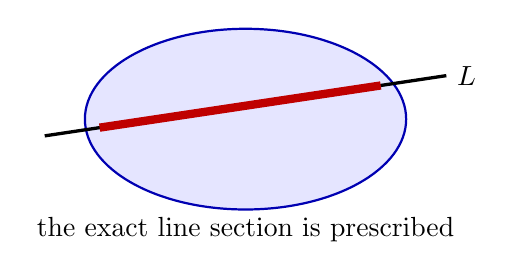
\begin{tikzpicture}[scale=.85]
  \fill[blue!10] (0,0) ellipse (2.4 and 1.35);
  \draw[blue!70!black,thick] (0,0) ellipse (2.4 and 1.35);
  \draw[very thick] (-3,-.25)--(3,.65) node[right] {$L$};
  \draw[red!75!black,line width=3pt] (-2.18,-.127)--(2.02,.503);
  \node at (0,-1.65) {the exact line section is prescribed};
\end{tikzpicture}

\caption{A prescribed line and its full bounded section.}
\end{subfigure}\hfill
\begin{subfigure}[t]{.47\textwidth}
\centering
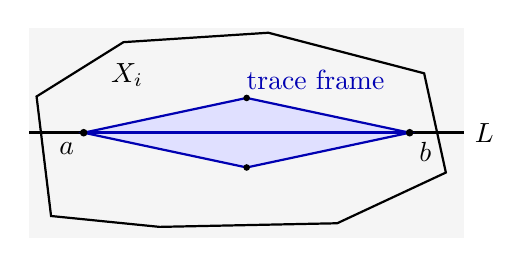
\begin{tikzpicture}[scale=.92]
  \fill[gray!8] (-3,-1.45) rectangle (3,1.45);
  \draw[thick] (-2.7,-1.15)--(-2.9,.5)--(-1.7,1.25)--(.3,1.38)--(2.45,.82)--(2.75,-.55)--(1.25,-1.25)--(-1.2,-1.3)--cycle;
  \draw[very thick] (-3,0)--(3,0) node[right] {$L$};
  \coordinate (a) at (-2.25,0); \coordinate (b) at (2.25,0);
  \coordinate (u) at (0,.48); \coordinate (d) at (0,-.48);
  \fill[blue!12] (a)--(u)--(b)--(d)--cycle;
  \draw[blue!70!black,thick] (a)--(u)--(b)--(d)--cycle;
  \draw[blue!70!black,very thick] (a)--(b);
  \fill (a) circle (1.5pt) node[below left] {$a$};
  \fill (b) circle (1.5pt) node[below right] {$b$};
  \fill (u) circle (1.3pt); \fill (d) circle (1.3pt);
  \node at (-1.65,.8) {$X_i$};
  \node[blue!70!black] at (.95,.73) {trace frame};
\end{tikzpicture}

\caption{A four-point trace frame freezes the section.}
\end{subfigure}
\caption{The uncut section is retained before the ambient polygon is
applied.}
\label{fig:traceframe}
\end{figure}

\subsection{The finite representative package}

Adjoin one ambient coordinate
\[
 U_0=\operatorname{int}F,\qquad X_0=F.
\]
Let $\mathcal L$ be the union of the prescribed lines and the finite
closure-degeneracy family $\mathcal L_{\rm deg}$.  Choose a finite set
$R$ containing:
\begin{enumerate}
\item one point of every atom of the closed tuple
      $(X_0,X_1,\ldots,X_n)$;
\item for every source open word, the vertices of a sufficiently small
      triangle lying in every active open field and containing a source
      witness of that word in its interior; every prescribed witness is
      used as the interior point of its triangle;
\item for every $L\in\mathcal L$ and every nonempty open section, all four
      vertices of a trace frame;
\item for every remaining nonempty closed section $L\cap X_i$, its extreme
      point or points;
\item every vertex of $F$.
\end{enumerate}
All data are finite.

\begin{theorem}[Finite-line relative polygonalization]\label{thm:main}
Let $F\subset\mathbb R^2$ be a compact convex polygon with nonempty
interior, let $U_1,\ldots,U_n$ be open convex sets, and let
$L_1,\ldots,L_m$ be finitely many affine lines.  Fix finitely many atom
witnesses in $\operatorname{int}F$.  Then there are compact convex polygons
$P_1,\ldots,P_n$ such that, with $V_i=\operatorname{int}P_i$:
\begin{enumerate}
\item the exact relative code is preserved,
\[
 \code(V_1\cap\operatorname{int}F,\ldots,
       V_n\cap\operatorname{int}F;\operatorname{int}F)
 =\code_F(\mathcal U);
\]
\item every prescribed strict trace is preserved,
\[
 L_s\cap V_i\cap F=L_s\cap U_i\cap F;
\]
\item simultaneously, every prescribed closed section is preserved,
\[
 L_s\cap P_i\cap F=L_s\cap\overline{U_i}\cap F;
\]
\item every protected witness remains in its original atom.
\end{enumerate}
The analogous statement holds in the relative affine hull when $F$ is a
segment or a point.
\end{theorem}

\begin{proof}
Apply \cref{lem:minimal} to the bounded closed tuple
$(X_0,X_1,\ldots,X_n)$ with the representative package $R$.  Let
$(Y_0,Y_1,\ldots,Y_n)$ be inclusion minimal.  Since $Y_0\subseteq F$ and
contains every vertex of $F$, one has $Y_0=F$.  By
\cref{lem:polygonal}, all remaining $Y_i$ are polygons, segments, points,
or empty.  Put $P_i=Y_i$ and $V_i=\operatorname{int}P_i$.

On every line in $\mathcal L_{\rm deg}$, the trace-frame and supporting
section data give the exact strict source trace.  The protected triangles
remain.  Hence \cref{lem:openrecovery} gives equality of the complete open
codes of
\[
 (\operatorname{int}F,V_1,\ldots,V_n)
 \quad\text{and}\quad
 (U_0,U_1\cap W,\ldots,U_n\cap W).
\]
Selecting the words containing the ambient coordinate gives the relative
code equality.  The same triangle argument preserves each protected
witness exactly.

Fix a prescribed line $L=L_s$ and a neuron $i$.  If the open bounded
section is $(a,b)$, the trace frame lies in $P_i$.  Every point of $(a,b)$
is interior to the quadrilateral and hence to $P_i$.  The endpoints cannot
be interior to $P_i\subseteq X_i$, and no point outside $[a,b]$ can enter
$P_i$.  Therefore
\[
 L\cap\operatorname{int}P_i=L\cap(U_i\cap W),
 \qquad L\cap P_i=L\cap X_i.
\]
If the open section is empty, \cref{lem:frame} gives the same two
identities.  Since $F\Subset W$,
\[
 X_i\cap F=\overline{U_i}\cap F,
\]
so clipping the identities by $F$ proves both prescribed trace clauses for
the original fields.

On a segment or point carrier, use the same construction in the relative
affine hull.  Inclusion-minimal compact convex sets there are intervals,
points, or empty.
\end{proof}

\begin{corollary}[Protected planar polygonalization]\label{cor:protected}
Every planar open convex code with finitely many designated atom witnesses
has a polygonal realization retaining those witnesses.
\end{corollary}

\begin{proof}
Choose a compact polygonal carrier containing the designated witnesses and
one witness for every codeword, and apply \cref{thm:main} with no prescribed
lines.
\end{proof}
